\chapter{Line Plots}\label{line-plots}

In this part, we will work towards creating the line plot below. We will
take you from a basic line plot and explain all the customisations we
add to the code step-by-step.

\begin{center}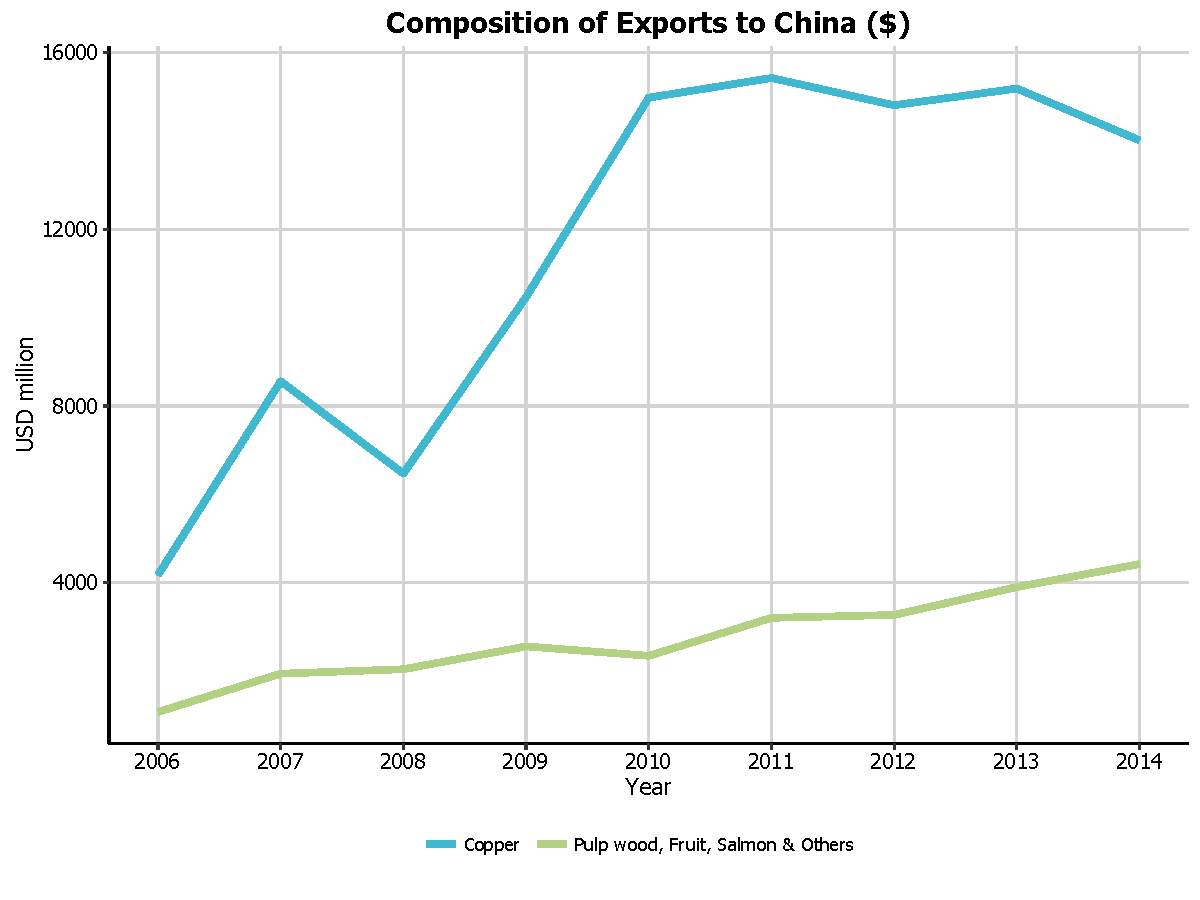
\includegraphics[width=0.55\linewidth]{figures/line_final-1} \end{center}

We will use an international trade \href{http://pachamaltese.github.io/stats/trade-chile-china/copper-data-for-tutorial.csv}{dataset} made by ourselves from different sources (Chile Customs,
Central Bank of Chile and General Directorate of International Economic Relations).

The first thing to do is load in the data and libraries, as below:

\begin{Shaded}
\begin{Highlighting}[]
\KeywordTok{library}\NormalTok{(ggplot2)}
\KeywordTok{library}\NormalTok{(ggthemes)}
\KeywordTok{library}\NormalTok{(extrafont)}

\NormalTok{charts.data <-}\StringTok{ }\KeywordTok{read.csv}\NormalTok{(}\StringTok{"copper-data-for-tutorial.csv"}\NormalTok{)}
\end{Highlighting}
\end{Shaded}

\section{Basic graph}\label{basic-graph}

In order to initialise a plot we tell ggplot that \texttt{charts.data}
is our data, and specify the variables on each axis. We then instruct
ggplot to render this as a line plot by adding the \texttt{geom\_line}
command.

\begin{Shaded}
\begin{Highlighting}[]
\NormalTok{p1 <-}\StringTok{ }\KeywordTok{ggplot}\NormalTok{() +}\StringTok{ }\KeywordTok{geom_line}\NormalTok{(}\KeywordTok{aes}\NormalTok{(}\DataTypeTok{y =} \NormalTok{export, }\DataTypeTok{x =} \NormalTok{year, }\DataTypeTok{colour =} \NormalTok{product), }
\StringTok{\StringTok{        }}\DataTypeTok{data =} \NormalTok{charts.data, }\DataTypeTok{stat=}\StringTok{"identity"}\NormalTok{)}
\NormalTok{p1}
\end{Highlighting}
\end{Shaded}

\begin{center}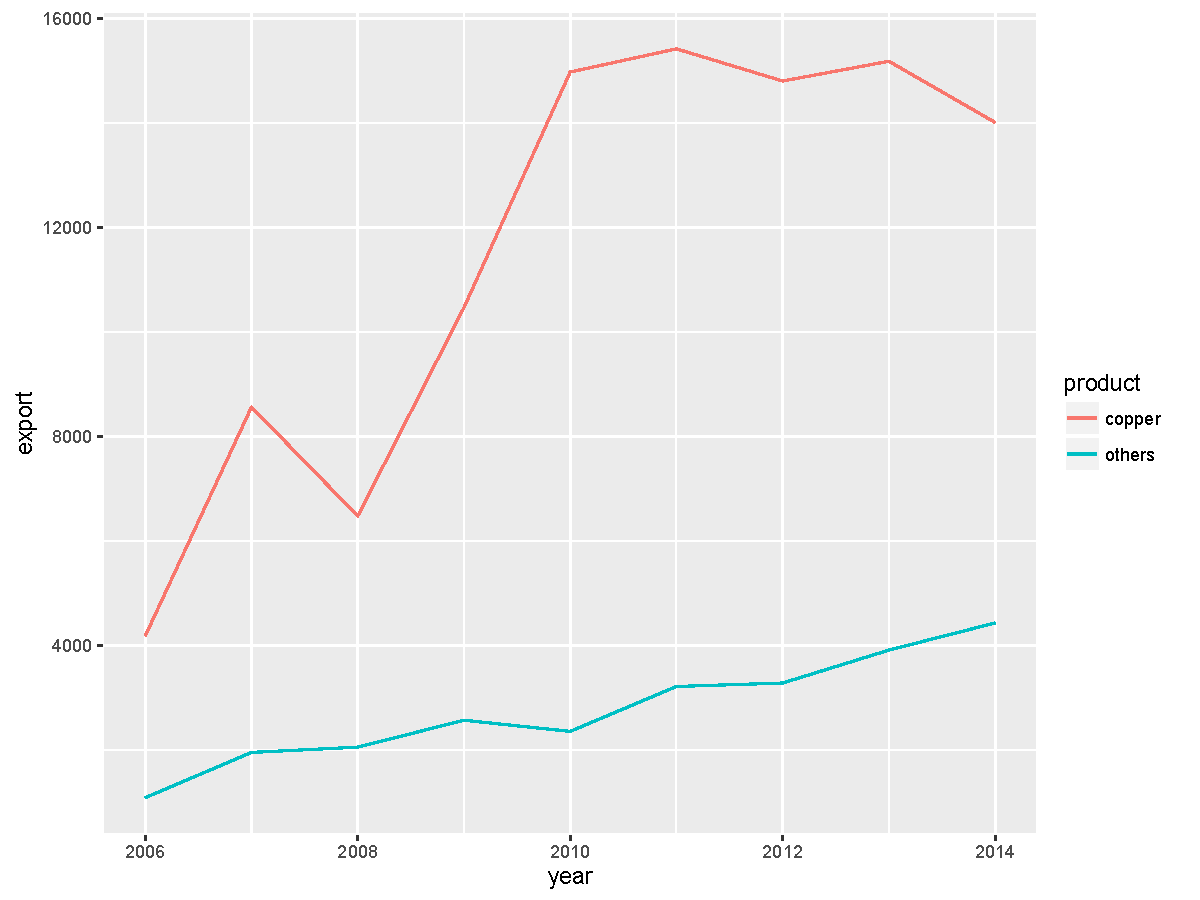
\includegraphics[width=0.55\linewidth]{figures/line_1-1} \end{center}

\section{Adjusting line width}\label{adjusting-line-width}

To change the line width, we add a \texttt{size} argument to
\texttt{geom\_line}.

\begin{Shaded}
\begin{Highlighting}[]
\NormalTok{p1 <-}\StringTok{ }\KeywordTok{ggplot}\NormalTok{() +}\StringTok{ }\KeywordTok{geom_line}\NormalTok{(}\KeywordTok{aes}\NormalTok{(}\DataTypeTok{y =} \NormalTok{export, }\DataTypeTok{x =} \NormalTok{year, }\DataTypeTok{colour =} \NormalTok{product), }
\StringTok{\StringTok{        }}\DataTypeTok{size=}\FloatTok{1.5}\NormalTok{, }\DataTypeTok{data =} \NormalTok{charts.data, }\DataTypeTok{stat=}\StringTok{"identity"}\NormalTok{)}
\NormalTok{p1}
\end{Highlighting}
\end{Shaded}

\begin{center}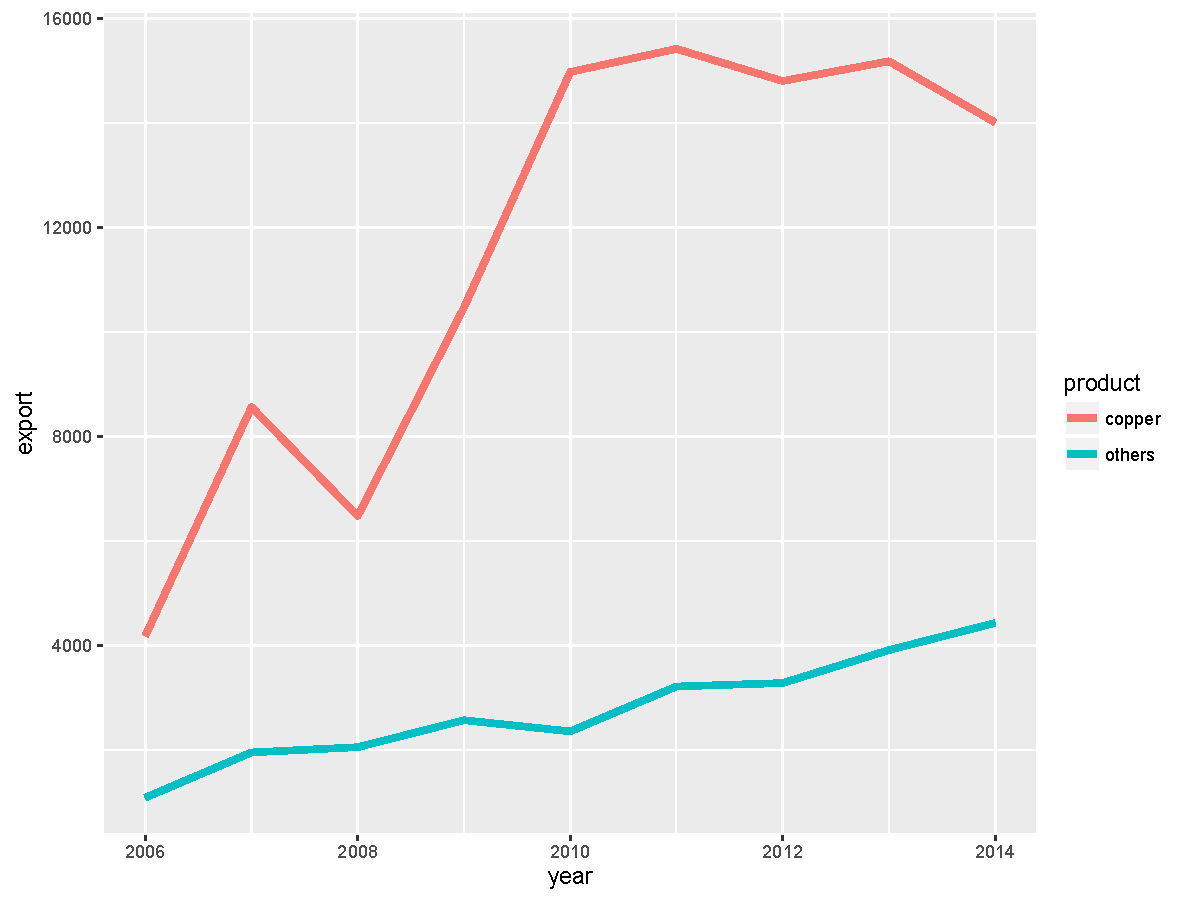
\includegraphics[width=0.55\linewidth]{figures/line_2-1} \end{center}

\section{Changing variables
display}\label{changing-variables-display}

To change the variables displayed name, we need to re-factor our data
labels in \texttt{charts.data} data frame. Then we move the legend to
the bottom using the \texttt{theme} command.

\begin{Shaded}
\begin{Highlighting}[]
\NormalTok{charts.data <-}\StringTok{ }\KeywordTok{as.data.frame}\NormalTok{(charts.data)}
\NormalTok{charts.data$product <-}\StringTok{ }\KeywordTok{factor}\NormalTok{(charts.data$product, }
\StringTok{\StringTok{        }}\DataTypeTok{levels =} \KeywordTok{c}\NormalTok{(}\StringTok{"copper"}\NormalTok{,}\StringTok{"others"}\NormalTok{), }
\StringTok{\StringTok{        }}\DataTypeTok{labels =} \KeywordTok{c}\NormalTok{(}\StringTok{"Copper"}\NormalTok{,}\StringTok{"Pulp wood, Fruit, Salmon & Others"}\NormalTok{))}

\NormalTok{p1 <-}\StringTok{ }\KeywordTok{ggplot}\NormalTok{() +}\StringTok{ }
\StringTok{      }\KeywordTok{geom_line}\NormalTok{(}\KeywordTok{aes}\NormalTok{(}\DataTypeTok{y =} \NormalTok{export, }\DataTypeTok{x =} \NormalTok{year, }\DataTypeTok{colour =} \NormalTok{product), }\DataTypeTok{size=}\FloatTok{1.5}\NormalTok{, }
\StringTok{\StringTok{        }}\DataTypeTok{data =} \NormalTok{charts.data, }\DataTypeTok{stat=}\StringTok{"identity"}\NormalTok{) +}
\StringTok{      }\KeywordTok{theme}\NormalTok{(}\DataTypeTok{legend.position=}\StringTok{"bottom"}\NormalTok{, }\DataTypeTok{legend.direction=}\StringTok{"horizontal"}\NormalTok{, }
\StringTok{\StringTok{        }}\DataTypeTok{legend.title =} \KeywordTok{element_blank}\NormalTok{())}
\NormalTok{p1}
\end{Highlighting}
\end{Shaded}

\begin{center}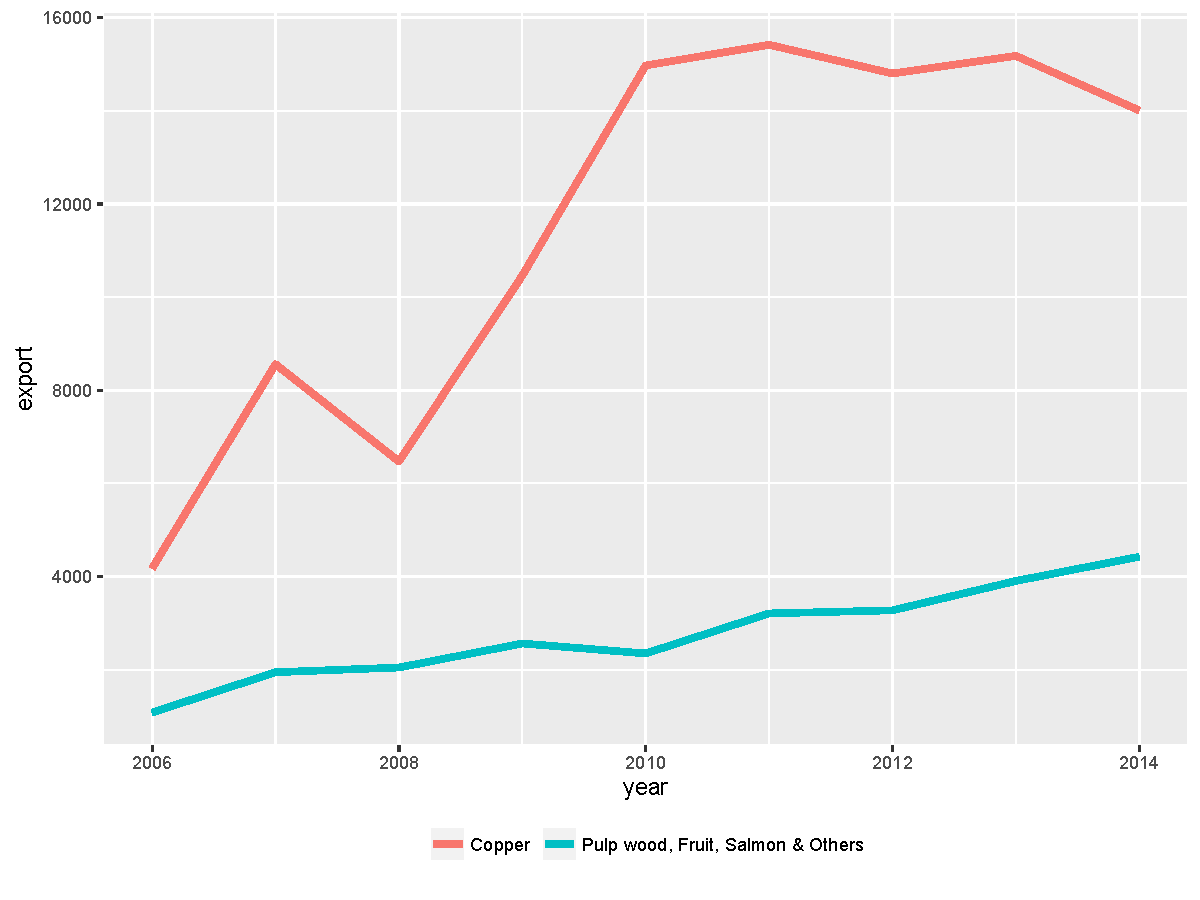
\includegraphics[width=0.55\linewidth]{figures/line_3-1} \end{center}

\section{Adjusting x-axis scale}\label{adjusting-x-axis-scale}

To change the axis tick marks, we use the \texttt{scale\_x\_continuous}
and/or \texttt{scale\_y\_continuous} commands.

\begin{Shaded}
\begin{Highlighting}[]
\NormalTok{p1 <-}\StringTok{ }\NormalTok{p1 +}\StringTok{ }\KeywordTok{scale_x_continuous}\NormalTok{(}\DataTypeTok{breaks=}\KeywordTok{seq}\NormalTok{(}\DecValTok{2006}\NormalTok{,}\DecValTok{2014}\NormalTok{,}\DecValTok{1}\NormalTok{))}
\NormalTok{p1}
\end{Highlighting}
\end{Shaded}

\begin{center}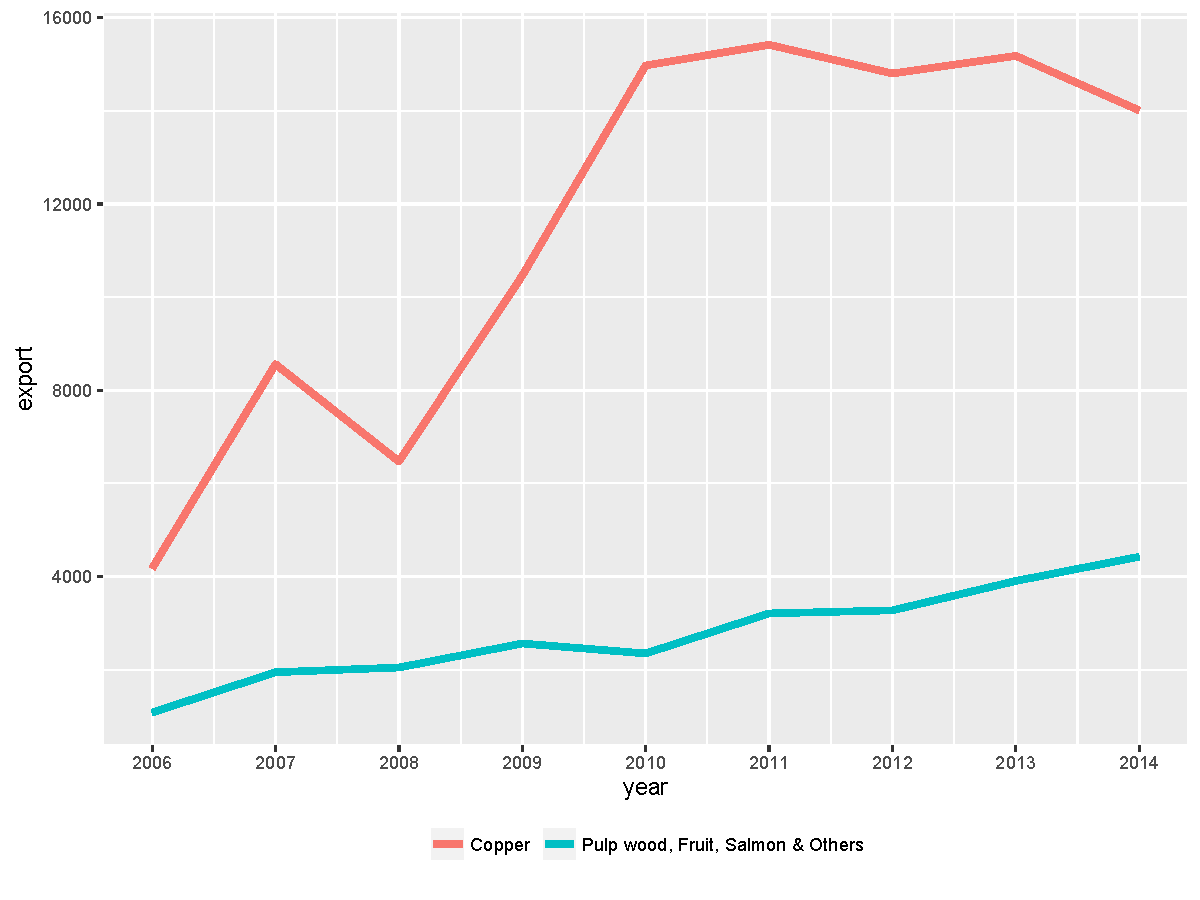
\includegraphics[width=0.55\linewidth]{figures/line_4-1} \end{center}

\section{Adjusting axis labels \& adding
title}\label{adjusting-axis-labels-adding-title}

To add a title, we include the option \texttt{ggtitle} and include the
name of the graph as a string argument, and to change the axis names we
use the \texttt{labs} command.

\begin{Shaded}
\begin{Highlighting}[]
\NormalTok{p1 <-}\StringTok{ }\NormalTok{p1 +}\StringTok{ }\KeywordTok{ggtitle}\NormalTok{(}\StringTok{"Composition of Exports to China ($)"}\NormalTok{) +}
\StringTok{      }\KeywordTok{labs}\NormalTok{(}\DataTypeTok{x=}\StringTok{"Year"}\NormalTok{, }\DataTypeTok{y=}\StringTok{"USD million"}\NormalTok{) }
\NormalTok{p1}
\end{Highlighting}
\end{Shaded}

\begin{center}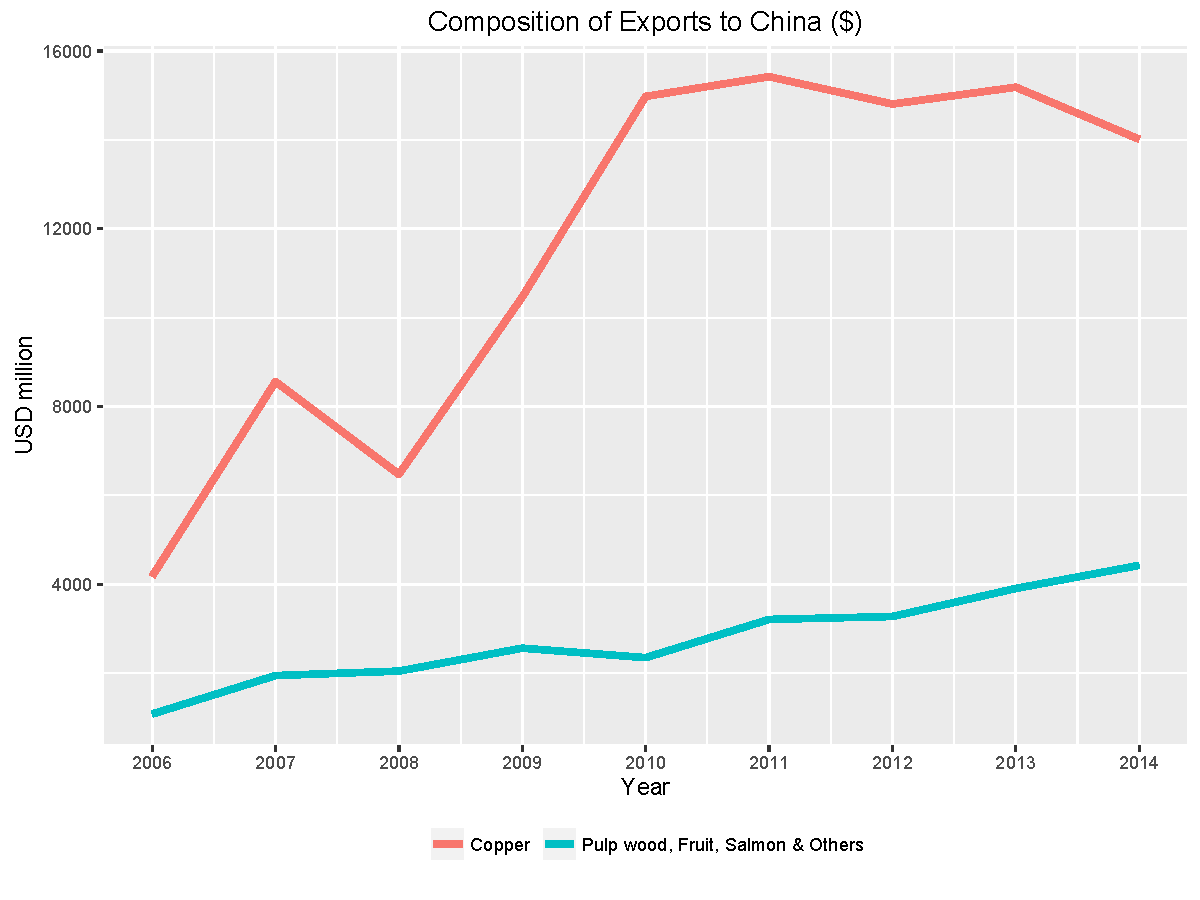
\includegraphics[width=0.55\linewidth]{figures/line_5-1} \end{center}

\section{Adjusting color palette}\label{adjusting-color-palette}

To change the colours, we use the \texttt{scale\_colour\_manual}
command.

\begin{Shaded}
\begin{Highlighting}[]
\NormalTok{colour <-}\StringTok{ }\KeywordTok{c}\NormalTok{(}\StringTok{"#5F9EA0"}\NormalTok{, }\StringTok{"#E1B378"}\NormalTok{)}
\NormalTok{p1 <-}\StringTok{ }\NormalTok{p1 +}\StringTok{ }\KeywordTok{scale_colour_manual}\NormalTok{(}\DataTypeTok{values=}\NormalTok{colour)}
\NormalTok{p1}
\end{Highlighting}
\end{Shaded}

\begin{center}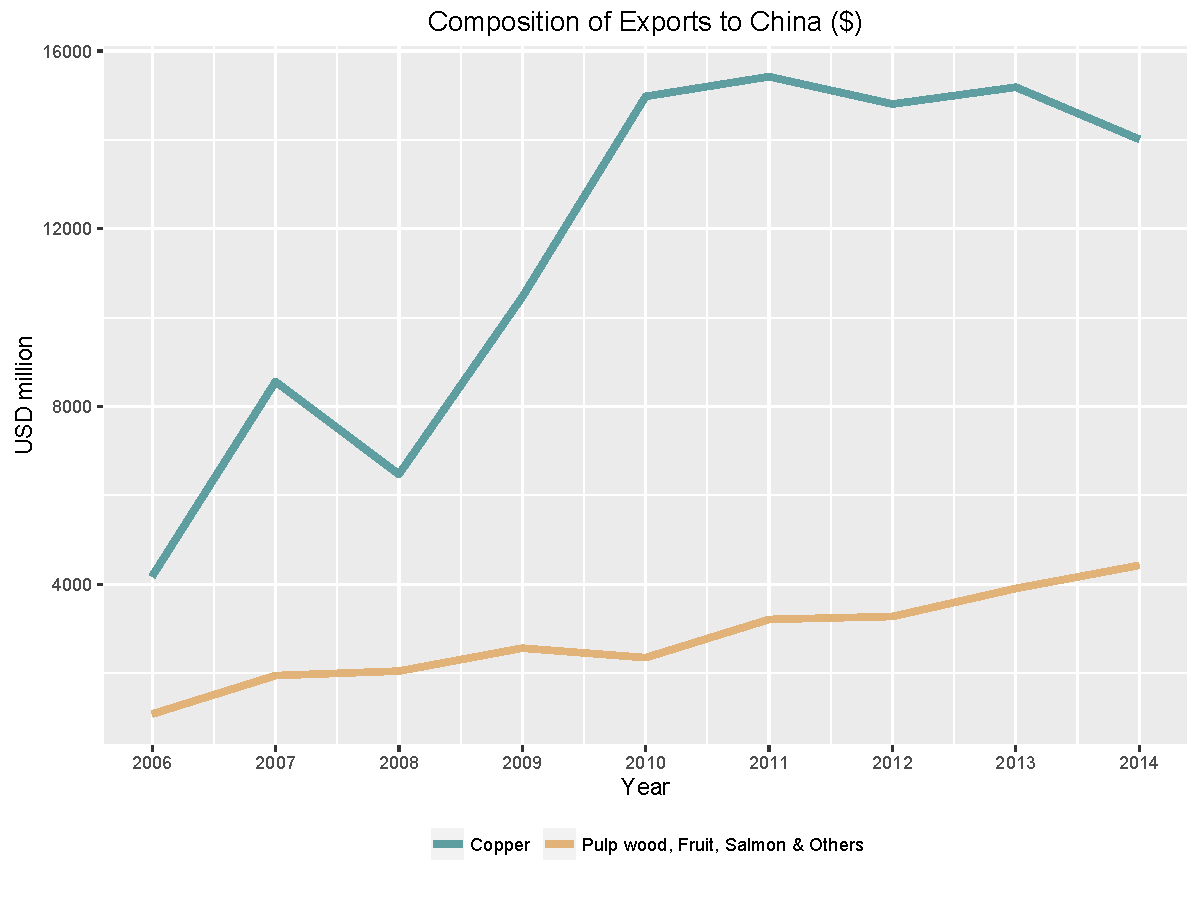
\includegraphics[width=0.55\linewidth]{figures/line_6-1} \end{center}

\section{Using the white theme}\label{using-the-white-theme}

We'll start using a simple theme customisation made adding
\texttt{theme\_bw()} after \texttt{ggplot()}. That theme argument can be
modified to use different themes.

\begin{Shaded}
\begin{Highlighting}[]
\NormalTok{p1 <-}\StringTok{ }\KeywordTok{ggplot}\NormalTok{() +}
\StringTok{      }\KeywordTok{geom_line}\NormalTok{(}\KeywordTok{aes}\NormalTok{(}\DataTypeTok{y =} \NormalTok{export, }\DataTypeTok{x =} \NormalTok{year, }\DataTypeTok{colour =} \NormalTok{product), }\DataTypeTok{size=}\FloatTok{1.5}\NormalTok{, }
\StringTok{\StringTok{        }}\DataTypeTok{data =} \NormalTok{charts.data, }\DataTypeTok{stat=}\StringTok{"identity"}\NormalTok{) +}\StringTok{ }
\StringTok{      }\KeywordTok{scale_x_continuous}\NormalTok{(}\DataTypeTok{breaks=}\KeywordTok{seq}\NormalTok{(}\DecValTok{2006}\NormalTok{,}\DecValTok{2014}\NormalTok{,}\DecValTok{1}\NormalTok{)) +}\StringTok{ }
\StringTok{      }\KeywordTok{labs}\NormalTok{(}\DataTypeTok{x=}\StringTok{"Year"}\NormalTok{, }\DataTypeTok{y=}\StringTok{"USD million"}\NormalTok{) +}\StringTok{ }
\StringTok{      }\KeywordTok{ggtitle}\NormalTok{(}\StringTok{"Composition of Exports to China ($)"}\NormalTok{) +}\StringTok{ }
\StringTok{      }\KeywordTok{scale_colour_manual}\NormalTok{(}\DataTypeTok{values=}\NormalTok{colour) +}
\StringTok{      }\KeywordTok{theme_bw}\NormalTok{() +}
\StringTok{      }\KeywordTok{theme}\NormalTok{(}\DataTypeTok{legend.position=}\StringTok{"bottom"}\NormalTok{, }
\StringTok{        }\DataTypeTok{legend.direction=}\StringTok{"horizontal"}\NormalTok{, }
\StringTok{        }\DataTypeTok{legend.title =} \KeywordTok{element_blank}\NormalTok{()) }
\NormalTok{p1}
\end{Highlighting}
\end{Shaded}

\begin{center}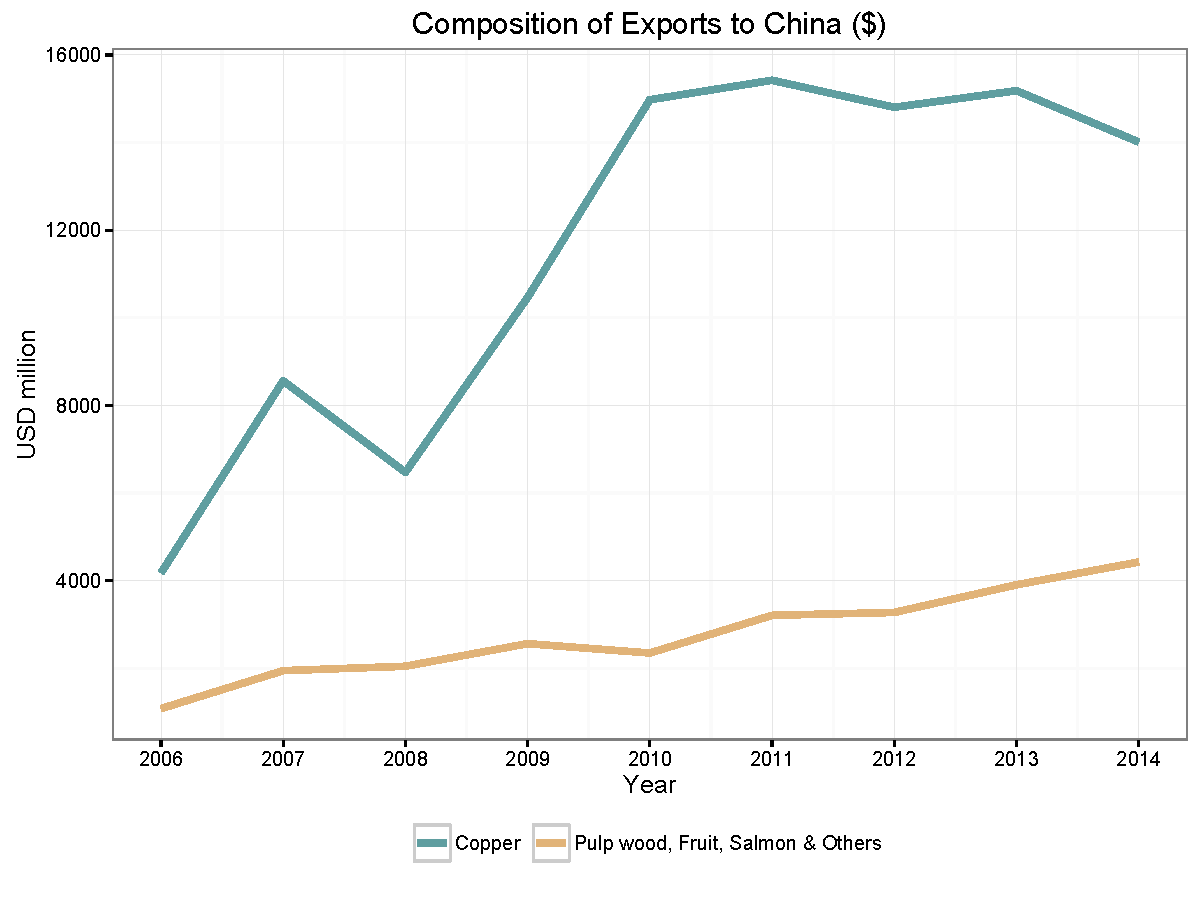
\includegraphics[width=0.55\linewidth]{figures/line_7-1} \end{center}

\section{Creating an XKCD style
chart}\label{creating-an-xkcd-style-chart}

Of course, you may want to create your own themes as well.
\texttt{ggplot2} allows for a very high degree of customisation,
including allowing you to use imported fonts. Below is an example of a
theme Mauricio was able to create which mimics the visual style of
\href{http://xkcd.com/}{XKCD}. In order to create this chart, you first
need to import the XKCD font, install it on your machine and load it
into R using the \texttt{extrafont} package. These instructions are
taken from
\href{https://www.google.com.au/url?sa=t\&rct=j\&q=\&esrc=s\&source=web\&cd=1\&ved=0ahUKEwiWzafchdPJAhVBpJQKHe_LDT8QFggbMAA\&url=https\%3A\%2F\%2Fcran.r-project.org\%2Fweb\%2Fpackages\%2Fxkcd\%2Fvignettes\%2Fxkcd-intro.pdf\&usg=AFQjCNE-KciGY14e-Q1buYIVmTFC0ht__Q\&sig2=DZUwkvIHwfNWtTtkcz94jg}{here}:

\begin{Shaded}
\begin{Highlighting}[]
\KeywordTok{library}\NormalTok{(extrafont)}

\KeywordTok{download.file}\NormalTok{(}\StringTok{"http://simonsoftware.se/other/xkcd.ttf"}\NormalTok{, }
\StringTok{      }\DataTypeTok{dest=}\StringTok{"xkcd.ttf"}\NormalTok{, }\DataTypeTok{mode=}\StringTok{"wb"}\NormalTok{)}
\KeywordTok{system}\NormalTok{(}\StringTok{"mkdir ~/.fonts"}\NormalTok{)}
\KeywordTok{system}\NormalTok{(}\StringTok{"cp xkcd.ttf  ~/.fonts"}\NormalTok{)}
\KeywordTok{font_import}\NormalTok{(}\DataTypeTok{paths =} \StringTok{"~/.fonts"}\NormalTok{, }\DataTypeTok{pattern=}\StringTok{"[X/x]kcd"}\NormalTok{)}
\KeywordTok{fonts}\NormalTok{()}
\KeywordTok{loadfonts}\NormalTok{()}
\end{Highlighting}
\end{Shaded}

You can then create your graph:

\begin{Shaded}
\begin{Highlighting}[]
\NormalTok{fill <-}\StringTok{ }\KeywordTok{c}\NormalTok{(}\StringTok{"#56B4E9"}\NormalTok{, }\StringTok{"#ff69b4"}\NormalTok{)}

\NormalTok{p1 <-}\StringTok{ }\KeywordTok{ggplot}\NormalTok{() +}\StringTok{ }
\StringTok{      }\KeywordTok{geom_line}\NormalTok{(}\KeywordTok{aes}\NormalTok{(}\DataTypeTok{y =} \NormalTok{export, }\DataTypeTok{x =} \NormalTok{year, }\DataTypeTok{colour =} \NormalTok{product), }\DataTypeTok{size=}\FloatTok{1.5}\NormalTok{, }
\StringTok{        }\DataTypeTok{data =} \NormalTok{charts.data, }\DataTypeTok{stat=}\StringTok{"identity"}\NormalTok{) +}\StringTok{ }
\StringTok{      }\KeywordTok{scale_x_continuous}\NormalTok{(}\DataTypeTok{breaks=}\KeywordTok{seq}\NormalTok{(}\DecValTok{2006}\NormalTok{,}\DecValTok{2014}\NormalTok{,}\DecValTok{1}\NormalTok{)) +}\StringTok{ }
\StringTok{      }\KeywordTok{labs}\NormalTok{(}\DataTypeTok{x=}\StringTok{"Year"}\NormalTok{, }\DataTypeTok{y=}\StringTok{"USD million"}\NormalTok{) +}\StringTok{ }
\StringTok{      }\KeywordTok{ggtitle}\NormalTok{(}\StringTok{"Composition of Exports to China ($)"}\NormalTok{) +}\StringTok{ }
\StringTok{      }\KeywordTok{scale_color_manual}\NormalTok{(}\DataTypeTok{values=}\NormalTok{fill) +}\StringTok{ }
\StringTok{      }\KeywordTok{theme}\NormalTok{(}\DataTypeTok{axis.text.x=}\KeywordTok{element_text}\NormalTok{(}\DataTypeTok{colour=}\StringTok{"black"}\NormalTok{, }\DataTypeTok{size =} \DecValTok{10}\NormalTok{), }
\StringTok{        }\DataTypeTok{axis.text.y=}\KeywordTok{element_text}\NormalTok{(}\DataTypeTok{colour=}\StringTok{"black"}\NormalTok{, }\DataTypeTok{size =} \DecValTok{10}\NormalTok{),}
\StringTok{        }\DataTypeTok{axis.line.x =} \KeywordTok{element_line}\NormalTok{(}\DataTypeTok{size=}\NormalTok{.}\DecValTok{5}\NormalTok{, }\DataTypeTok{colour =} \StringTok{"black"}\NormalTok{),}
\StringTok{        }\DataTypeTok{axis.line.y =} \KeywordTok{element_line}\NormalTok{(}\DataTypeTok{size=}\NormalTok{.}\DecValTok{5}\NormalTok{, }\DataTypeTok{colour =} \StringTok{"black"}\NormalTok{),}
\StringTok{        }\DataTypeTok{legend.key=}\KeywordTok{element_rect}\NormalTok{(}\DataTypeTok{fill=}\StringTok{"white"}\NormalTok{, }\DataTypeTok{colour=}\StringTok{"white"}\NormalTok{),}
\StringTok{        }\DataTypeTok{legend.position=}\StringTok{"bottom"}\NormalTok{, }\DataTypeTok{legend.direction=}\StringTok{"horizontal"}\NormalTok{, }
\StringTok{        }\DataTypeTok{legend.title =} \KeywordTok{element_blank}\NormalTok{(),}
\StringTok{        }\DataTypeTok{panel.grid.major =} \KeywordTok{element_blank}\NormalTok{(),}
\StringTok{        }\DataTypeTok{panel.grid.minor =} \KeywordTok{element_blank}\NormalTok{(), }\DataTypeTok{panel.border =} \KeywordTok{element_blank}\NormalTok{(), }
\StringTok{        }\DataTypeTok{panel.background =} \KeywordTok{element_blank}\NormalTok{(),}
\StringTok{        }\DataTypeTok{plot.title=}\KeywordTok{element_text}\NormalTok{(}\DataTypeTok{family=}\StringTok{"xkcd-Regular"}\NormalTok{), }
\StringTok{        }\DataTypeTok{text=}\KeywordTok{element_text}\NormalTok{(}\DataTypeTok{family=}\StringTok{"xkcd-Regular"}\NormalTok{)) }
\NormalTok{p1}
\end{Highlighting}
\end{Shaded}

\begin{center}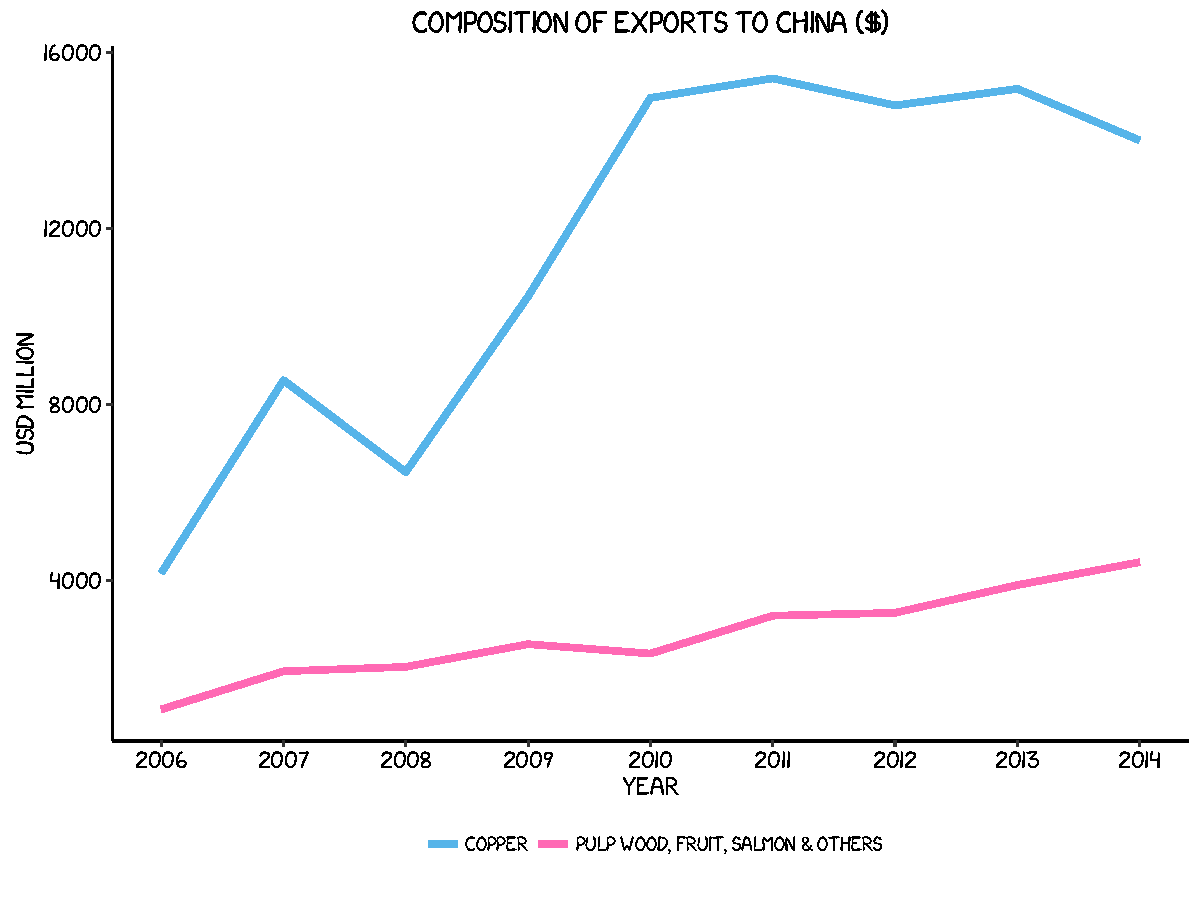
\includegraphics[width=0.55\linewidth]{figures/line_8-1} \end{center}

\section{\texorpdfstring{Using `The Economist'
theme}{Using The Economist theme}}\label{using-the-economist-theme}

There are a wider range of pre-built themes available as part of the
\texttt{ggthemes} package (more information on these
\href{https://cran.r-project.org/web/packages/ggthemes/vignettes/ggthemes.html}{here}).
Below we've applied \texttt{theme\_economist()}, which approximates
graphs in the Economist magazine. It is also important that the font
change argument inside \texttt{theme} is optional and it's only to
obtain a more similar result compared to the original. For an exact
result you need `Officina Sans' which is a commercial font and is
available \href{http://www.myfonts.com/fonts/itc/officina-sans/}{here}.

\begin{Shaded}
\begin{Highlighting}[]
\NormalTok{p1 <-}\StringTok{ }\KeywordTok{ggplot}\NormalTok{() +}
\StringTok{      }\KeywordTok{geom_line}\NormalTok{(}\KeywordTok{aes}\NormalTok{(}\DataTypeTok{y =} \NormalTok{export, }\DataTypeTok{x =} \NormalTok{year, }\DataTypeTok{colour =} \NormalTok{product), }\DataTypeTok{size=}\FloatTok{1.5}\NormalTok{, }
\StringTok{        }\DataTypeTok{data =} \NormalTok{charts.data, }\DataTypeTok{stat=}\StringTok{"identity"}\NormalTok{) +}\StringTok{ }
\StringTok{      }\KeywordTok{scale_x_continuous}\NormalTok{(}\DataTypeTok{breaks=}\KeywordTok{seq}\NormalTok{(}\DecValTok{2006}\NormalTok{,}\DecValTok{2014}\NormalTok{,}\DecValTok{1}\NormalTok{)) +}\StringTok{ }
\StringTok{      }\KeywordTok{labs}\NormalTok{(}\DataTypeTok{x=}\StringTok{"Year"}\NormalTok{, }\DataTypeTok{y=}\StringTok{"USD million"}\NormalTok{) +}\StringTok{ }
\StringTok{      }\KeywordTok{ggtitle}\NormalTok{(}\StringTok{"Composition of Exports to China ($)"}\NormalTok{) +}
\StringTok{      }\KeywordTok{theme_economist}\NormalTok{() +}\StringTok{ }\KeywordTok{scale_colour_economist}\NormalTok{() +}
\StringTok{      }\KeywordTok{theme}\NormalTok{(}\DataTypeTok{axis.line.x =} \KeywordTok{element_line}\NormalTok{(}\DataTypeTok{size=}\NormalTok{.}\DecValTok{5}\NormalTok{, }\DataTypeTok{colour =} \StringTok{"black"}\NormalTok{), }
\StringTok{        }\DataTypeTok{axis.line.y =} \KeywordTok{element_line}\NormalTok{(}\DataTypeTok{size=}\NormalTok{.}\DecValTok{5}\NormalTok{, }\DataTypeTok{colour =} \StringTok{"black"}\NormalTok{),}
\StringTok{        }\DataTypeTok{legend.position=}\StringTok{"bottom"}\NormalTok{, }
\StringTok{        }\DataTypeTok{legend.direction=}\StringTok{"horizontal"}\NormalTok{, }
\StringTok{        }\DataTypeTok{legend.title =} \KeywordTok{element_blank}\NormalTok{(),}
\StringTok{        }\DataTypeTok{plot.title=}\KeywordTok{element_text}\NormalTok{(}\DataTypeTok{family=}\StringTok{"OfficinaSanITC-Book"}\NormalTok{),}
\StringTok{        }\DataTypeTok{text=}\KeywordTok{element_text}\NormalTok{(}\DataTypeTok{family=}\StringTok{"OfficinaSanITC-Book"}\NormalTok{)) }
\NormalTok{p1}
\end{Highlighting}
\end{Shaded}

\begin{center}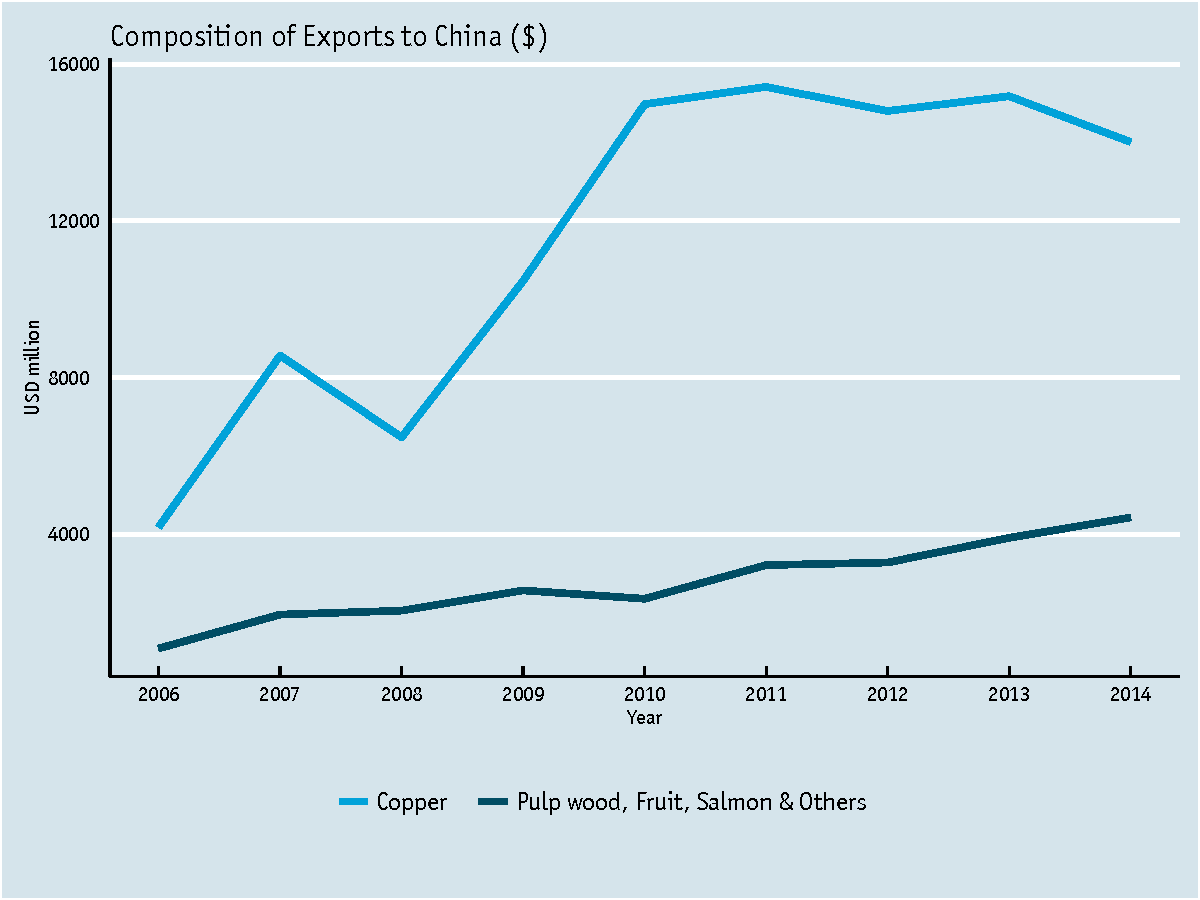
\includegraphics[width=0.55\linewidth]{figures/line_9-1} \end{center}

\section{Creating your own theme}\label{creating-your-own-theme}

As before, you can modify your plots a lot as \texttt{ggplot2} allows
many customisations. Here we present our original result shown at the
top of page.

\begin{Shaded}
\begin{Highlighting}[]
\NormalTok{colour <-}\StringTok{ }\KeywordTok{c}\NormalTok{(}\StringTok{"#40b8d0"}\NormalTok{, }\StringTok{"#b2d183"}\NormalTok{)}

\NormalTok{p1 <-}\StringTok{ }\KeywordTok{ggplot}\NormalTok{() +}\StringTok{ }
\StringTok{      }\KeywordTok{geom_line}\NormalTok{(}\KeywordTok{aes}\NormalTok{(}\DataTypeTok{y =} \NormalTok{export, }\DataTypeTok{x =} \NormalTok{year, }\DataTypeTok{colour =} \NormalTok{product), }\DataTypeTok{size=}\FloatTok{1.5}\NormalTok{, }
\StringTok{        }\DataTypeTok{data =} \NormalTok{charts.data, }\DataTypeTok{stat=}\StringTok{"identity"}\NormalTok{) +}\StringTok{ }
\StringTok{      }\KeywordTok{scale_x_continuous}\NormalTok{(}\DataTypeTok{breaks=}\KeywordTok{seq}\NormalTok{(}\DecValTok{2006}\NormalTok{,}\DecValTok{2014}\NormalTok{,}\DecValTok{1}\NormalTok{)) +}\StringTok{ }
\StringTok{      }\KeywordTok{labs}\NormalTok{(}\DataTypeTok{x=}\StringTok{"Year"}\NormalTok{, }\DataTypeTok{y=}\StringTok{"USD million"}\NormalTok{) +}\StringTok{ }
\StringTok{      }\KeywordTok{ggtitle}\NormalTok{(}\StringTok{"Composition of Exports to China ($)"}\NormalTok{) +}\StringTok{ }
\StringTok{      }\KeywordTok{scale_colour_manual}\NormalTok{(}\DataTypeTok{values=}\NormalTok{colour) +}\StringTok{ }
\StringTok{      }\KeywordTok{theme}\NormalTok{(}\DataTypeTok{axis.line.x =} \KeywordTok{element_line}\NormalTok{(}\DataTypeTok{size=}\NormalTok{.}\DecValTok{5}\NormalTok{, }\DataTypeTok{colour =} \StringTok{"black"}\NormalTok{), }
\StringTok{        }\DataTypeTok{axis.line.y =} \KeywordTok{element_line}\NormalTok{(}\DataTypeTok{size=}\NormalTok{.}\DecValTok{5}\NormalTok{, }\DataTypeTok{colour =} \StringTok{"black"}\NormalTok{), }
\StringTok{        }\DataTypeTok{axis.text.x=}\KeywordTok{element_text}\NormalTok{(}\DataTypeTok{colour=}\StringTok{"black"}\NormalTok{, }\DataTypeTok{size =} \DecValTok{10}\NormalTok{), }
\StringTok{        }\DataTypeTok{axis.text.y=}\KeywordTok{element_text}\NormalTok{(}\DataTypeTok{colour=}\StringTok{"black"}\NormalTok{, }\DataTypeTok{size =} \DecValTok{10}\NormalTok{),}
\StringTok{        }\DataTypeTok{legend.key=}\KeywordTok{element_rect}\NormalTok{(}\DataTypeTok{fill=}\StringTok{"white"}\NormalTok{, }\DataTypeTok{colour=}\StringTok{"white"}\NormalTok{),}
\StringTok{        }\DataTypeTok{legend.position=}\StringTok{"bottom"}\NormalTok{, }\DataTypeTok{legend.direction=}\StringTok{"horizontal"}\NormalTok{, }
\StringTok{        }\DataTypeTok{legend.title =} \KeywordTok{element_blank}\NormalTok{(),}
\StringTok{        }\DataTypeTok{panel.grid.major =} \KeywordTok{element_line}\NormalTok{(}\DataTypeTok{colour =} \StringTok{"#d3d3d3"}\NormalTok{), }
\StringTok{        }\DataTypeTok{panel.grid.minor =} \KeywordTok{element_blank}\NormalTok{(), }
\StringTok{        }\DataTypeTok{panel.border =} \KeywordTok{element_blank}\NormalTok{(), }
\StringTok{        }\DataTypeTok{panel.background =} \KeywordTok{element_blank}\NormalTok{(),}
\StringTok{        }\DataTypeTok{plot.title =} \KeywordTok{element_text}\NormalTok{(}\DataTypeTok{size =} \DecValTok{14}\NormalTok{, }\DataTypeTok{family =} \StringTok{"Tahoma"}\NormalTok{, }\DataTypeTok{face =} \StringTok{"bold"}\NormalTok{), }
\StringTok{        }\DataTypeTok{text=}\KeywordTok{element_text}\NormalTok{(}\DataTypeTok{family=}\StringTok{"Tahoma"}\NormalTok{)) }
\NormalTok{p1}
\end{Highlighting}
\end{Shaded}

\begin{center}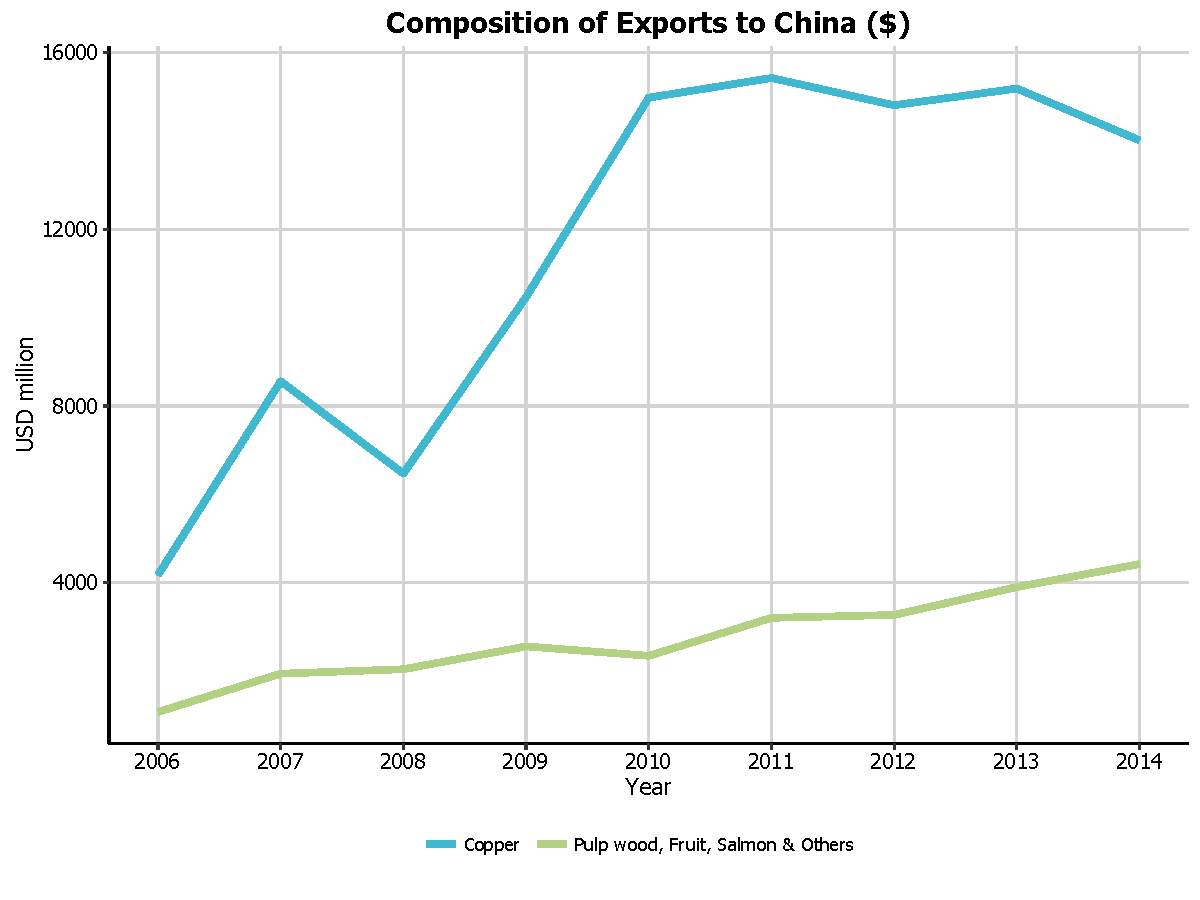
\includegraphics[width=0.55\linewidth]{figures/line_11-1} \end{center}